% Provenance (never printed): see sources/outline_sources.md (Year 1: stress and
% principal stresses in 2D; strain; pure and simple shear; elastic, brittle and ductile
% behaviour; the strength envelope of the lithosphere). Strength envelopes from
% figdata/bachelor-1/strength_envelope.py (Byerlee 1975; flow laws of Gleason and Tullis
% 1995 and Hirth and Kohlstedt 2003 as compiled by Lopez-Sanchez; geotherms of ch. 10);
% exercise and problem values in the Book 3 scratch calculator calc/ch16.py. Traction,
% shear stress, the stress and strain tensors, Hooke's law, Young's modulus and viscosity
% belong to the physics series and are recalled, never defined (sync 1 ruling).
\chapter{Spanning, rek en reologie}\label{ch:b1:stress-strain-rheology}

In de jaren zestig stroomde afvalvloeistof die in een injectieput bij het Rocky Mountain Arsenal, nabij Denver, werd geperst, door gebarsten kristallijn fundamentgesteente tussen \qty{3.7}{km} en \qty{7.0}{km} onder het oppervlak, en er volgden aardbevingen. Zij bleven binnen het deel van de rots waar de vloeistofdruk met meer dan ongeveer \qty{3.2}{MPa} was gestegen.
% ledger: hb81:denver
Een halve eeuw later gebeurde hetzelfde op grotere schaal in Oklahoma, waar zout water dat met olie en gas naar boven komt, weer de grond in wordt gepompt. In en rond de staat waren er aardbevingen van magnitude 3 of meer: één tot vijf per jaar van 2005 tot 2008, daarna \num{20} in 2009, \num{585} in 2014 en \num{888} in 2015, meer dan twee per dag. Schokken van magnitude 5.7 en 5.8 schudden Praag in 2011 en Pawnee in 2016. Vier injectieputten met een groot volume konden alleen al een vijfde van de aardbevingen in het midden van de Verenigde Staten verklaren, en sommige veroorzaakten schokken meer dan \qty{30}{km} verder weg.
% ledger: usgs:oklahoma-rate, usgs:prague-pawnee, keranen:oklahoma
Het water duwde niets opzij; het verhoogde alleen de druk van de vloeistof in de poriën van het gesteente. Waarom zou dat een breuk doen schuiven? Het antwoord vraagt drie ideeën, het onderwerp van dit hoofdstuk: de spanning op een vlak in een gesteente, de voorwaarde waaronder het vlak bezwijkt, en het feit dat de druk van de poriënvloeistof tegenwerkt tegen de kracht die de twee zijden tegen elkaar drukt. Met die drie, en met een kruipwet voor heet gesteente, kunnen we de sterkte van de hele \omterm{def:b1:layered-earth:lithosphere}{lithosfeer} tegen de diepte uitzetten.

\begin{recall}
Een kracht die over een oppervlak is verdeeld, werkt via haar kracht per oppervlakte-eenheid, in pascal; de druk in een vloeistof in rust neemt met de diepte toe als $\rho g z$ (natuurkunde, eerste jaar universiteit). Een veer en een vaste stof bij kleine vervormingen gehoorzamen aan de wet van Hooke: de rek is evenredig met de spanning, met de elasticiteitsmodulus van Young als constante; een viskeuze vloeistof weerstaat in verhouding tot haar afschuifsnelheid, met haar viscositeit als constante. Het natuurkundeboek voor het derde jaar beschrijft spanning en rek in drie dimensies met tensoren; dit hoofdstuk heeft er maar twee nodig. Een symmetrische $2\times2$-matrix heeft twee reële eigenwaarden en twee loodrechte eigenvectoren (wiskunde, eerste jaar universiteit). De \omterm{def:b1:heat-budget:geotherm}{geotherm} van \cref{ch:b1:heat-budget} geven de temperatuur met de diepte; breuken kwamen in Boek 1, klas 7 aan bod.
\end{recall}

\section{Spanning in twee dimensies}\label{sec:b1:stress-strain-rheology:stress}

Snijd in gedachten een rots door langs een klein plat vlak. De rots aan de ene kant drukt op de rots aan de andere kant met een kracht, en de kracht per oppervlakte-eenheid is de traktie op dat vlak, het woord van de natuurkundeboeken. Haar richting is in het algemeen niet de richting van de normaal op het vlak.

\begin{definition}[Normaalspanning]\label{def:b1:stress-strain-rheology:stress}
Op een vlak door een punt van een rots is de kracht per oppervlakte-eenheid die de rots aan de ene kant op de andere uitoefent, een component langs de normaal op het vlak, de \emph{normaalspanning}\index{normaalspanning} $\sigma_n$, en een component langs het vlak, de schuifspanning $\tau$. In de aardwetenschappen telt de normaalspanning positief wanneer zij drukt.
\end{definition}

De tekenconventie is het omgekeerde van die van de ingenieur. Zij is gekozen omdat bijna elke spanning in de vaste Aarde een drukspanning is: het gewicht van de rots erboven drukt op alles eronder.

We werken in een verticaal vlak, met een horizontale as $x$ en een as $y$. Op een vlak loodrecht op $x$ zijn de \omterm{def:b1:stress-strain-rheology:stress}{normaalspanning} $\sigma_{xx}$ en de schuifspanning $\sigma_{xy}$; op een vlak loodrecht op $y$ zijn dat $\sigma_{yy}$ en $\sigma_{yx}$. De twee schuifspanningen zijn gelijk: op een klein vierkantje maken de schuifkrachten op de verticale zijden een koppel met moment $\sigma_{xy}a\cdot a$ voor een zijde $a$, die op de horizontale zijden een koppel $\sigma_{yx}a\cdot a$ dat de andere kant op draait, en het vierkantje zou gaan draaien als zij verschilden. Zo beschrijven drie getallen de spanning in een punt, en die zijn genoeg om haar op elk vlak te geven.

\begin{proposition}[Spanning op een schuin vlak]\label{prop:b1:stress-strain-rheology:transformation}
Laat een vlak de eenheidsnormaal $\vec n = (\cos\theta, \sin\theta)$ hebben, onder de hoek $\theta$ met de as $x$, en laat $\vec m = (-\sin\theta, \cos\theta)$ de eenheidsvector langs het vlak zijn. De normaal- en schuifspanning erop zijn
\begin{align*}
  \sigma_n &= \sigma_{xx}\cos^2\theta + 2\sigma_{xy}\sin\theta\cos\theta + \sigma_{yy}\sin^2\theta
           = \frac{\sigma_{xx}+\sigma_{yy}}{2} + \frac{\sigma_{xx}-\sigma_{yy}}{2}\cos2\theta + \sigma_{xy}\sin2\theta, \\
  \tau     &= (\sigma_{yy}-\sigma_{xx})\sin\theta\cos\theta + \sigma_{xy}(\cos^2\theta - \sin^2\theta)
           = -\frac{\sigma_{xx}-\sigma_{yy}}{2}\sin2\theta + \sigma_{xy}\cos2\theta ,
\end{align*}
waarbij $\tau$ positief wordt geteld langs $\vec m$.
\end{proposition}

\begin{proof}
Snijd een klein prisma uit, zoals in de figuur hieronder: een schuin vlak met oppervlak $A$ en buitenwaartse normaal $\vec n$, een verticaal vlak met oppervlak $A\cos\theta$ en een horizontaal vlak met oppervlak $A\sin\theta$, per eenheid van lengte in de derde richting. Zijn gewicht en zijn traagheid schalen met zijn volume, dat sneller krimpt dan zijn vlakken; voor een voldoende klein prisma moeten de krachten op de vlakken dus op zichzelf in evenwicht zijn. Omdat drukspanning positief is, duwt de rots van buitenaf op het verticale vlak met de kracht $A\cos\theta\,(\sigma_{xx}, \sigma_{xy})$ en op het horizontale vlak met $A\sin\theta\,(\sigma_{xy}, \sigma_{yy})$; op het schuine vlak duwt zij met $-A(\sigma_n\vec n + \tau\vec m)$. De som is nul:
\[
  \sigma_n\vec n + \tau\vec m = \cos\theta\,(\sigma_{xx}, \sigma_{xy}) + \sin\theta\,(\sigma_{xy}, \sigma_{yy}) .
\]
Het scalair product met $\vec n$ geeft $\sigma_n$, dat met $\vec m$ geeft $\tau$, omdat $\vec n\cdot\vec m = 0$. De tweede vormen volgen uit $\cos^2\theta = (1+\cos2\theta)/2$, $\sin^2\theta = (1-\cos2\theta)/2$ en $2\sin\theta\cos\theta = \sin2\theta$.
\end{proof}

\begin{omfigure}
\begin{tikzpicture}[>={Stealth[length=5pt]}, font=\small]
% theta = 35 deg, hypotenuse L = 4.5: a = L cos(theta), b = L sin(theta)
\pgfmathsetmacro{\th}{35}
\pgfmathsetmacro{\L}{4.5}
\pgfmathsetmacro{\a}{\L*cos(\th)}
\pgfmathsetmacro{\b}{\L*sin(\th)}
\coordinate (O) at (0,0);
\coordinate (A) at (0,\a);
\coordinate (B) at (\b,0);
\coordinate (M) at ($(A)!0.5!(B)$);
\fill[omLithGranite!45] (O) -- (A) -- (B) -- cycle;
\draw[line width=0.8pt] (O) -- (A) -- (B) -- cycle;
% axes
\draw[->, black!70] (-2.6,-1.9) -- (-1.6,-1.9) node[right] {$x$};
\draw[->, black!70] (-2.6,-1.9) -- (-2.6,-0.9) node[above] {$y$};
% face on x = 0 (outward normal -x), area A cos(theta)
\draw[->, line width=1.1pt, omDef] (-1.35,0.5*\a) -- (-0.05,0.5*\a);
\node[omDef, anchor=south] at (-0.95,0.5*\a+0.05) {$\sigma_{xx} A\cos\theta$};
\draw[->, line width=1.1pt, omProp] (-0.25,0.5*\a-1.25) -- (-0.25,0.5*\a-0.25);
\node[omProp, anchor=east] at (-0.3,0.5*\a-0.85) {$\sigma_{xy} A\cos\theta$};
% face on y = 0 (outward normal -y), area A sin(theta)
\draw[->, line width=1.1pt, omDef] (0.68*\b,-1.35) -- (0.68*\b,-0.05);
\node[omDef, anchor=west] at (0.68*\b+0.05,-1.05) {$\sigma_{yy} A\sin\theta$};
\draw[->, line width=1.1pt, omProp] (0.1,-0.25) -- (1.1,-0.25);
\node[omProp, anchor=north east] at (0.9,-0.32) {$\sigma_{xy} A\sin\theta$};
% inclined face, area A, normal n = (cos theta, sin theta)
\draw[->, line width=1.1pt, omThm] ($(M)+(\th:1.5)$) -- ($(M)+(\th:0.05)$);
\node[omThm, anchor=south west, inner sep=1pt] at ($(M)+(\th:1.5)$) {$\sigma_n A$};
\draw[->, line width=1.1pt, omThm!70!black] ($(M)+(\th:0.25)+(\th-90:0.75)$) -- ($(M)+(\th:0.25)+(\th-90:1.75)$);
\node[omThm!70!black, anchor=west] at ($(M)+(\th:0.3)+(\th-90:1.3)$) {$\tau A$};
\draw[->, black!70, dashed] ($(M)+(\th+90:1.25)$) -- ++(\th:1.0) node[pos=1, anchor=south west, inner sep=1pt, text=black] {$\boldsymbol n$};
% angle theta at A, between the face and the y axis
\pic[draw, angle radius=0.75cm, pic text={$\theta$}, angle eccentricity=1.35] {angle = O--A--B};
\end{tikzpicture}
\par\smallskip{\small Het krachtenevenwicht op een klein driehoekig prisma van rots. Het schuine vlak heeft oppervlak $A$ en eenheidsnormaal $\vec n$; het verticale en het horizontale vlak hebben de oppervlakken $A\cos\theta$ en $A\sin\theta$. Blauw: de normaalkrachten op de twee kleine vlakken; oranje: de schuifkrachten erop; rood: de normaal- en schuifkrachten op het schuine vlak. Drukspanning telt positief, dus elke normaalkracht wijst het prisma in.}
\label{fig:b1:stress-strain-rheology:prism}
\end{omfigure}

\begin{theorem}[Hoofdspanningen]\label{thm:b1:stress-strain-rheology:principal}
Op elk punt van een rots zijn er twee loodrechte vlakken waarop de schuifspanning nul is. De \omterm{def:b1:stress-strain-rheology:stress}{normaalspanningen} op die vlakken zijn de grootste en de kleinste \omterm{def:b1:stress-strain-rheology:stress}{normaalspanning} over alle vlakken door het punt,
\[
  \sigma_{1,3} = \frac{\sigma_{xx}+\sigma_{yy}}{2} \pm
  \sqrt{\Bigl(\frac{\sigma_{xx}-\sigma_{yy}}{2}\Bigr)^2 + \sigma_{xy}^2},
  \qquad \tan2\theta_p = \frac{2\sigma_{xy}}{\sigma_{xx}-\sigma_{yy}},
\]
waarbij $\theta_p$ de hoek is van de as $x$ tot de normaal van het vlak dat $\sigma_1$ draagt.
\end{theorem}

\begin{proof}
Schrijf $c = (\sigma_{xx}+\sigma_{yy})/2$, en kies $R \ge 0$ en $\theta_p$ met $(\sigma_{xx}-\sigma_{yy})/2 = R\cos2\theta_p$ en $\sigma_{xy} = R\sin2\theta_p$; dan
$R = \sqrt{((\sigma_{xx}-\sigma_{yy})/2)^2 + \sigma_{xy}^2}$ en $\tan2\theta_p$ is zoals vermeld. De tweede vormen van \cref{prop:b1:stress-strain-rheology:transformation} worden
\[
  \sigma_n = c + R\cos(2\theta - 2\theta_p), \qquad \tau = -R\sin(2\theta - 2\theta_p).
\]
De \omterm{def:b1:stress-strain-rheology:stress}{normaalspanning} is het grootst, $c + R$, voor $\theta = \theta_p$, en het kleinst, $c - R$, voor $\theta = \theta_p + \ang{90}$; op beide is $\tau = 0$. Let ook op dat $\mathrm d\sigma_n/\mathrm d\theta = 2\tau$: de \omterm{def:b1:stress-strain-rheology:stress}{normaalspanning} is stationair precies waar de schuifspanning verdwijnt.
\end{proof}

\begin{definition}[Hoofdspanningen, differentiële spanning]\label{def:b1:stress-strain-rheology:principal}
De \emph{hoofdspanningen}\index{hoofdspanningen} in een punt zijn de \omterm{def:b1:stress-strain-rheology:stress}{normaalspanningen} $\sigma_1 \ge \sigma_3$ op de twee vlakken zonder schuifspanning, en hun richtingen zijn de hoofdrichtingen. In drie dimensies zijn er drie, $\sigma_1 \ge \sigma_2 \ge \sigma_3$, op drie loodrechte vlakken. De \emph{differentiële spanning}\index{differentiële spanning} is $\sigma_1 - \sigma_3$, en de gemiddelde spanning in het vlak is $(\sigma_1+\sigma_3)/2$.
\end{definition}

Een spanningstoestand is het gemakkelijkst af te lezen in haar hoofdrichtingen. Meten we de hoek $\theta$ vanaf de richting van $\sigma_1$ in plaats van vanaf de as $x$, dan vallen de laatste termen van de formules weg.

\begin{proposition}[Cirkel van Mohr]\label{prop:b1:stress-strain-rheology:mohr}
Op een vlak waarvan de normaal de hoek $\theta$ maakt met de richting van $\sigma_1$,
\[
  \sigma_n = \frac{\sigma_1+\sigma_3}{2} + \frac{\sigma_1-\sigma_3}{2}\cos2\theta,
  \qquad
  |\tau| = \frac{\sigma_1-\sigma_3}{2}\,|\sin2\theta| .
\]
Wanneer $\theta$ draait, doorloopt het punt $(\sigma_n, |\tau|)$ de bovenhelft van de cirkel met middelpunt $((\sigma_1+\sigma_3)/2,\, 0)$ en straal $(\sigma_1-\sigma_3)/2$, onder de hoek $2\theta$ vanaf zijn $\sigma_1$-einde. De grootste schuifspanning, $(\sigma_1-\sigma_3)/2$, werkt op de vlakken onder \ang{45} met de hoofdrichtingen.
\end{proposition}

\begin{proof}
In de hoofdassen geldt $\sigma_{xx} = \sigma_1$, $\sigma_{yy} = \sigma_3$ en $\sigma_{xy} = 0$, en \cref{prop:b1:stress-strain-rheology:transformation} geeft de twee formules. Dan volgt $(\sigma_n - (\sigma_1+\sigma_3)/2)^2 + \tau^2 = ((\sigma_1-\sigma_3)/2)^2$, de vergelijking van de cirkel; $|\sin2\theta|$ is het grootst voor $\theta = \ang{45}$.
\end{proof}

Het teken van $\tau$ zegt alleen in welke zin de twee zijden zouden glijden, daarom wordt meestal alleen de bovenhelft van de cirkel getekend. De constructie is genoemd naar de ingenieur Christian Otto Mohr, die er ook een bezwijkcriterium op bouwde; daar gaan we naartoe (\cref{sec:b1:stress-strain-rheology:rheology}).

\subsection*{Spanning op diepte}

\begin{definition}[Lithostatische druk, poriënvloeistofdruk, effectieve spanning]\label{def:b1:stress-strain-rheology:lithostatic}
Op diepte $z$ is het gewicht van de rots erboven, per eenheid van horizontaal oppervlak, de verticale spanning $\sigma_v = \int_0^z\rho g\,\mathrm dz'$, die gelijk is aan $\rho g z$ in een laag van uniforme dichtheid $\rho$.
Wanneer de spanning in elke richting dezelfde is en gelijk aan de verticale spanning, zit de rots onder de \emph{lithostatische druk}\index{lithostatische druk}. De druk van het water, de olie of het gas in de poriën en scheurtjes van de rots is de \emph{poriënvloeistofdruk}\index{poriënvloeistofdruk} $P$; zij is hydrostatisch, $P = \rho_w g z$, wanneer de poriën met het oppervlak verbonden zijn. De \emph{effectieve spanning}\index{effectieve spanning} is de spanning min de poriëndruk, $\sigma' = \sigma - P$, op elk vlak; $\lambda = P/\sigma_v$ is de poriëndrukverhouding.
\end{definition}

In een \omterm{def:b1:layered-earth:layers}{korst} met dichtheid \qty{2700}{kg.m^{-3}} neemt de verticale spanning met $2700\times9.81\times1000 = \qty{26.5}{MPa}$ per kilometer toe, en de hydrostatische poriëndruk met \qty{9.81}{MPa} per kilometer: $\lambda = 1000/2700 = 0.37$.
De poriënvloeistof duwt de korrels met dezelfde druk in elke richting uiteen; zij neemt niets van de schuifspanning weg, maar zij neemt $P$ van elke \omterm{def:b1:stress-strain-rheology:stress}{normaalspanning} af. Waar de poriën zijn afgesloten, bijvoorbeeld door klei of zout, kan de vloeistof een deel van het gewicht van de rots erboven dragen, en $\lambda$ stijgt naar 1.

De spanning in de \omterm{def:b1:layered-earth:layers}{korst} is niet lithostatisch. Platen duwen en trekken, de \omterm{def:b1:layered-earth:layers}{korst} buigt, bergen wegen op hun wortels, en de horizontale spanningen verschillen van de verticale. Nabij het oppervlak, dat geen schuifspanning draagt, is een hoofdrichting verticaal, zoals \cref{ch:b1:faults-folds-fabrics} laat zien: $\sigma_v$ is $\sigma_1$, $\sigma_2$ of $\sigma_3$, en de drie gevallen zijn de drie manieren waarop breuken bewegen.

\section{Rek}\label{sec:b1:stress-strain-rheology:strain}

Spanning is een oorzaak; rek is wat de rots registreert. Een uitgerekt fossiel, een afgeplatte kiezel en een laag die tot \omterm{def:b1:geological-maps:fold}{plooien} is ingekort, meten alle een verandering van vorm.

\begin{definition}[Verlenging, strekking, schuifrek]\label{def:b1:stress-strain-rheology:strain}
Een lijn van materiaal met lengte $\ell_0$ die wordt vervormd tot lengte $\ell$, heeft de \emph{verlenging}\index{verlenging (rek)} $e = (\ell - \ell_0)/\ell_0$ en de \emph{strekking}\index{strekking} $S = \ell/\ell_0 = 1 + e$; een verkorting is een negatieve verlenging, een strekking kleiner dan 1. Twee lijnen van materiaal die loodrecht stonden en nu de hoek $\ang{90} - \psi$ maken, zijn over de hoek $\psi$ geschoven, en de \emph{schuifrek}\index{schuifrek} is $\gamma = \tan\psi$.
\end{definition}

Een rek is homogeen wanneer elk klein gebied van de rots op dezelfde manier vervormt. De nieuwe positie $\vec x'$ van het punt $\vec x$ is dan een lineaire functie, $\vec x' = F\vec x$, met een constante $2\times2$-matrix $F$ (en $\det F > 0$, omdat een rots zich niet binnenstebuiten keert). Rechte lijnen blijven recht en evenwijdige lijnen evenwijdig; een vierkant wordt een parallellogram, en een cirkel wordt een ellips.

\begin{proposition}[De rekellips]\label{prop:b1:stress-strain-rheology:ellipse}
Onder de homogene rek $\vec x' = F\vec x$ wordt de cirkel met straal 1 een ellips waarvan de halve assen de vierkantswortels $S_1 \ge S_2$ zijn van de eigenwaarden van $FF^{\mathsf T}$, langs haar loodrechte eigenvectoren. $S_1$ en $S_2$ zijn de grootste en de kleinste \omterm{def:b1:stress-strain-rheology:strain}{strekking} van alle lijnen van materiaal, en het oppervlak wordt vermenigvuldigd met $\det F = S_1S_2$.
\end{proposition}

\begin{proof}
Het punt $\vec x = F\vec u$ komt van een punt $\vec u$ van de cirkel, $|\vec u| = 1$, dus $|F^{-1}\vec x|^2 = 1$, dat wil zeggen $\vec x^{\mathsf T}(FF^{\mathsf T})^{-1}\vec x = 1$. De matrix $B = FF^{\mathsf T}$ is symmetrisch met positieve eigenwaarden $\lambda_1 \ge
\lambda_2$ ($\vec v^{\mathsf T}B\vec v = |F^{\mathsf T}\vec v|^2 > 0$); in haar loodrechte eigenvectoren luidt de vergelijking $x_1^2/\lambda_1 + x_2^2/\lambda_2 = 1$, een ellips met halve assen $\sqrt{\lambda_1}$ en $\sqrt{\lambda_2}$. Een lijn van materiaal langs de eenheidsvector $\vec u$ heeft de \omterm{def:b1:stress-strain-rheology:strain}{strekking} $|F\vec u|$, en $|F\vec u|^2 = \vec u^{\mathsf T}F^{\mathsf T}F\vec u$ ligt tussen de eigenwaarden van $F^{\mathsf T}F$, die dezelfde zijn als die van $FF^{\mathsf T}$. Ten slotte is $\lambda_1\lambda_2 = \det B = (\det F)^2$.
\end{proof}

\begin{definition}[Rekellips]\label{def:b1:stress-strain-rheology:strain-ellipse}
De \emph{rekellips}\index{rekellips} is de ellips waarin een homogene rek een cirkel met straal 1 verandert; haar halve assen zijn de hoofdstrekkingen $S_1 \ge S_2$, en haar assen zijn de hoofdrichtingen van de rek.
\end{definition}

Twee rekken die de vorm van een lichaam even sterk veranderen, kunnen heel verschillend zijn.

\begin{definition}[Zuivere schuif, eenvoudige schuif]\label{def:b1:stress-strain-rheology:shear-types}
Een \emph{zuivere schuif}\index{zuivere schuif} is een homogene rek die het oppervlak behoudt en haar hoofdrichtingen vastlegt in de rots: $F = \begin{pmatrix} k & 0 \\ 0 & 1/k\end{pmatrix}$ in die assen, met $k > 1$. Een \emph{eenvoudige schuif}\index{eenvoudige schuif} verplaatst elk punt evenwijdig aan één richting, de schuifrichting, met $\gamma$ maal zijn afstand tot een vast vlak evenwijdig eraan: $F = \begin{pmatrix} 1 & \gamma \\ 0 & 1\end{pmatrix}$.
\end{definition}

Beide behouden het oppervlak, want beide determinanten zijn 1. Bij \omterm{def:b1:stress-strain-rheology:shear-types}{zuivere schuif} blijven de lijnen van materiaal langs de assen van de \omterm{def:b1:stress-strain-rheology:strain-ellipse}{rekellips} dezelfde lijnen in elke fase: de rek is coaxiaal. Bij \omterm{def:b1:stress-strain-rheology:shear-types}{eenvoudige schuif} is dat niet zo, zoals de volgende propositie en de figuur erna laten zien.

\begin{proposition}[De ellips van eenvoudige schuif]\label{prop:b1:stress-strain-rheology:simple-shear}
Een \omterm{def:b1:stress-strain-rheology:shear-types}{eenvoudige schuif} $\gamma$ heeft de hoofdstrekkingen
\[
  S_{1,2} = \sqrt{1 + \gamma^2/4} \pm \gamma/2 ,
\]
en de lange as van haar \omterm{def:b1:stress-strain-rheology:strain-ellipse}{rekellips} maakt met de schuifrichting de hoek $\theta'$ gegeven door $\tan2\theta' = 2/\gamma$.
\end{proposition}

\begin{proof}
$FF^{\mathsf T} = \begin{pmatrix} 1+\gamma^2 & \gamma \\ \gamma & 1\end{pmatrix}$
heeft spoor $2+\gamma^2$ en determinant 1. Dus $S_1S_2 = 1$ en $S_1^2 + S_2^2 = 2 + \gamma^2$, zodat $(S_1 - S_2)^2 = \gamma^2$, $S_1 - S_2 = \gamma$, en $S_1 = \gamma/2 + \sqrt{1+\gamma^2/4}$. De eigenvector van de grootste eigenwaarde van een symmetrische matrix $\begin{pmatrix} a & b \\ b & d\end{pmatrix}$ maakt met de eerste as de hoek gegeven door $\tan2\theta' = 2b/(a-d)$ (\cref{thm:b1:stress-strain-rheology:principal} is dezelfde berekening): hier $2\gamma/\gamma^2 = 2/\gamma$.
\end{proof}

\begin{omfigure}
\begin{tikzpicture}[>={Stealth[length=4.5pt]}, font=\small, scale=0.95]
% unit square [-1,1]^2 with its inscribed circle, mapped by exact linear maps (cm = a,b,c,d: x' = a x + c y, y' = b x + d y)
% pure shear: diag(k, 1/k), k = (1 + sqrt 5)/2 = 1.618; simple shear: gamma = 1, S1 = 1.618, long axis at 31.72 deg
\pgfmathsetmacro{\k}{(1+sqrt(5))/2}
\pgfmathsetmacro{\ik}{1/\k}
% (a) undeformed
\begin{scope}
  \fill[omLithSand!70] (-1,-1) rectangle (1,1);
  \draw[line width=0.7pt] (-1,-1) rectangle (1,1);
  \draw[line width=0.9pt, omDef] (0,0) circle[radius=1];
  \draw[omThm, line width=0.6pt] (-1,-1) -- (1,1);
  \draw[omProp, line width=0.6pt] (-1,1) -- (1,-1);
  \node[font=\small\bfseries] at (0,-1.55) {(a) voor};
\end{scope}
% (b) pure shear
\begin{scope}[xshift=4.2cm]
  \draw[black!35, dashed] (-1,-1) rectangle (1,1);
  \begin{scope}[cm={\k,0,0,\ik,(0,0)}]
    \fill[omLithSand!70] (-1,-1) rectangle (1,1);
    \draw[line width=0.7pt] (-1,-1) rectangle (1,1);
    \draw[line width=0.9pt, omDef] (0,0) circle[radius=1];
    \draw[omThm, line width=0.6pt] (-1,-1) -- (1,1);
    \draw[omProp, line width=0.6pt] (-1,1) -- (1,-1);
  \end{scope}
  \draw[omDef, dashed] (-\k,0) -- (\k,0);
  \draw[omDef, dashed] (0,-\ik) -- (0,\ik);
  \draw[->, line width=0.8pt] (1.72,0) -- (2.15,0);
  \draw[->, line width=0.8pt] (-1.72,0) -- (-2.15,0);
  \draw[->, line width=0.8pt] (0,1.2) -- (0,0.72);
  \draw[->, line width=0.8pt] (0,-1.2) -- (0,-0.72);
  \node[font=\small\bfseries] at (0,-1.55) {(b) zuivere schuif};
\end{scope}
% (c) simple shear, gamma = 1
\begin{scope}[xshift=9.0cm]
  \draw[black!35, dashed] (-1,-1) rectangle (1,1);
  \begin{scope}[cm={1,0,1,1,(0,0)}]
    \fill[omLithSand!70] (-1,-1) rectangle (1,1);
    \draw[line width=0.7pt] (-1,-1) rectangle (1,1);
    \draw[line width=0.9pt, omDef] (0,0) circle[radius=1];
    \draw[omThm, line width=0.6pt] (-1,-1) -- (1,1);
    \draw[omProp, line width=0.6pt] (-1,1) -- (1,-1);
  \end{scope}
  % long and short axes of the strain ellipse: S1 = 1.618 at 31.72 deg, S2 = 0.618 at 121.72 deg
  \draw[omDef, dashed] (211.72:\k) -- (31.72:\k);
  \draw[omDef, dashed] (121.72:\ik) -- (301.72:\ik);
  \draw[->, line width=0.8pt] (-1.2,1.3) -- (0.8,1.3);
  \draw[->, line width=0.8pt] (1.2,-1.3) -- (-0.8,-1.3);
  \draw[black!60] (-2,-1) -- (-2,0.2);
  \draw[black!70] (-2,-0.3) arc[start angle=90, end angle=45, radius=0.7];
  \node[font=\scriptsize] at ($(-2,-1)+(67.5:0.98)$) {$\psi$};
  \node[font=\small\bfseries] at (0,-1.75) {(c) eenvoudige schuif};
\end{scope}
\end{tikzpicture}
\par\smallskip{\small Een vierkant van rots met de ingeschreven cirkel (a), vervormd door een \omterm{def:b1:stress-strain-rheology:shear-types}{zuivere schuif} met $k = 1.618$ (b) en door een \omterm{def:b1:stress-strain-rheology:shear-types}{eenvoudige schuif} met $\gamma = 1$ (c), die dezelfde hoofdstrekkingen hebben, 1.618 en 0.618. Blauw gestreept: de assen van de \omterm{def:b1:stress-strain-rheology:strain-ellipse}{rekellips}; grijs gestreept: het vierkant ervoor. Bij \omterm{def:b1:stress-strain-rheology:shear-types}{zuivere schuif} blijven de assen op dezelfde lijnen van materiaal; bij \omterm{def:b1:stress-strain-rheology:shear-types}{eenvoudige schuif} ligt de lange as op \ang{31.7} van de schuifrichting, en de diagonaal die aan het begin de richting van de snelste rek was (rood), is er al voorbij gedraaid, tot \ang{26.6}. De vormen zijn exacte beelden van het vierkant en de cirkel onder de twee matrices.}
\label{fig:b1:stress-strain-rheology:shear}
\end{omfigure}

De \omterm{def:b1:stress-strain-rheology:strain-ellipse}{rekellips} legt de totale, of \emph{eindige}, rek vast. Een vervorming die miljoenen jaren duurt, is de som van veel kleine toenames, elk een oneindig kleine rek; voor een kleine $\gamma$ geeft de propositie $S_{1,2} \approx 1 \pm \gamma/2$ en $\theta' \approx \ang{45}$. Bij \omterm{def:b1:stress-strain-rheology:shear-types}{eenvoudige schuif} strekken de toenames altijd het snelst onder \ang{45} met de schuifrichting, terwijl de eindige ellips ernaartoe draait: \ang{31.7} bij $\gamma = 1$, \ang{22.5} bij $\gamma = 2$, steeds dichter erbij naarmate $\gamma$ groeit. Daarom liggen afgeplatte kiezels en uitgerekte mineralen in een zone van sterke schuif bijna in haar vlak, en meet de hoek die zij met de zone maken hoe ver zij is verschoven.

\section{Reologie}\label{sec:b1:stress-strain-rheology:rheology}

\begin{definition}[Reologie, bros en taai gedrag]\label{def:b1:stress-strain-rheology:rheology}
De \emph{reologie}\index{reologie} van een materiaal is de manier waarop het vervormt en stroomt onder spanning: het verband tussen spanning, rek en de snelheid van de rek. Een rots vertoont \emph{bros gedrag}\index{bros gedrag} wanneer zij vervormt door breuk of door schuiven langs breuken, op afzonderlijke vlakken, met een plotseling verlies van sterkte; zij vertoont \emph{taai gedrag}\index{taai gedrag} wanneer zij permanent en continu door haar volume vervormt, zonder haar samenhang te verliezen.
\end{definition}

Rotsen vertonen alle gedragingen die in de natuurkundeboeken worden behandeld. Onder kleine, korte spanningen zijn zij elastisch: de rek is evenredig met de spanning, zoals in de wet van Hooke, en verdwijnt samen met haar; seismische golven (\cref{ch:b1:layered-earth}) reizen door elastische rots. Over lange tijden stroomt de hete \omterm{def:b1:layered-earth:layers}{mantel} als een zeer viskeuze vloeistof, waarbij de snelheid van de rek toeneemt met de spanning. Daartussen breekt koude rots en glijdt zij, en kruipt warme rots. Welk gedrag de overhand krijgt, hangt af van de spanning, de temperatuur, de druk, de vloeistof in de poriën en de beschikbare tijd.

\subsection*{Bros bezwijken}

\begin{definition}[Coulomb-bezwijkcriterium]\label{def:b1:stress-strain-rheology:coulomb}
Een rots gehoorzaamt aan het \emph{Coulomb-bezwijkcriterium}\index{Coulomb-bezwijkcriterium} wanneer een erdoorheen gelegd vlak breekt, of een bestaande breuk schuift, zodra op dat vlak
\[
  \tau = C + \mu\,\sigma_n' , \qquad \sigma_n' = \sigma_n - P ,
\]
waarbij $C \ge 0$ de \emph{cohesie}\index{cohesie} van de rots is, $\mu$ haar \emph{inwendige wrijvingscoëfficiënt}\index{inwendige wrijvingscoëfficiënt} en $\phi = \arctan\mu$ haar \emph{inwendige wrijvingshoek}\index{inwendige wrijvingshoek}.
\end{definition}

Het criterium draagt de namen van Coulomb en Mohr. Zijn constanten worden in het laboratorium op monsters gemeten en verschillen van gesteente tot gesteente. Een bestaande breuk heeft haar \omterm{def:b1:stress-strain-rheology:coulomb}{cohesie} verloren: voor haar geldt $C = 0$, en de wrijving erop hangt nauwelijks van het gesteente af (\cref{prop:b1:stress-strain-rheology:byerlee}), met $\mu$ tussen 0.6 en 0.85, een wrijvingshoek tussen \ang{31} en \ang{40}.
% ledger: byerlee:1975

\begin{theorem}[De bezwijkhoek]\label{thm:b1:stress-strain-rheology:failure-angle}
Een rots die aan het Coulomb-criterium gehoorzaamt, bezwijkt eerst op de vlakken die de hoek $\ang{45} - \phi/2$ maken met de richting van $\sigma_1$, aan weerszijden ervan, en zij bezwijkt wanneer
\[
  \frac{\sigma_1' - \sigma_3'}{2} = C\cos\phi + \frac{\sigma_1' + \sigma_3'}{2}\,\sin\phi .
\]
\end{theorem}

\begin{proof}
Teken de cirkel van Mohr in \omterm{def:b1:stress-strain-rheology:lithostatic}{effectieve spanningen}, met middelpunt $c' =
(\sigma_1'+\sigma_3')/2$ en straal $r = (\sigma_1'-\sigma_3')/2$
(figuur hieronder); de poriëndruk heeft hem met $P$ verschoven, want zij neemt $P$ van elke \omterm{def:b1:stress-strain-rheology:stress}{normaalspanning} af en niets van de schuifspanning. Zolang de hele cirkel onder de lijn $\tau = C + \mu\sigma_n'$ ligt,
breekt geen vlak. Wanneer de spanningen veranderen, is het eerste vlak dat breekt het punt waar de cirkel de lijn raakt. Daar staat de straal loodrecht op de lijn; de lijn stijgt onder de hoek $\phi$ boven de horizontale, zodat de straal naar het raakpunt de hoek $\ang{90} + \phi$ maakt met de richting van het $\sigma_1$-einde. Volgens \cref{prop:b1:stress-strain-rheology:mohr} is dit punt het vlak waarvan de normaal de hoek $\theta$ maakt met $\sigma_1$, waarbij $2\theta = \ang{90} + \phi$; het vlak zelf maakt $\ang{90} - \theta = \ang{45} - \phi/2$ met $\sigma_1$, en de onderste helft van de cirkel geeft het symmetrische vlak. Raken betekent dat de afstand van het middelpunt tot de lijn gelijk is aan de straal: $r = (C + \mu c')/\sqrt{1+\mu^2} = C\cos\phi + c'\sin\phi$, omdat $\cos\phi = 1/\sqrt{1+\mu^2}$ en $\sin\phi = \mu/\sqrt{1+\mu^2}$.
\end{proof}

\begin{omfigure}
\begin{tikzpicture}[>={Stealth[length=5pt]}, font=\small, x=0.072cm, y=0.072cm]
% C = 10 MPa, mu = 0.6 (phi = 30.96 deg), sigma_3' = 20 MPa; tangency r = (C + mu sigma_3') / (sqrt(1+mu^2) - mu)
\pgfmathsetmacro{\C}{10}
\pgfmathsetmacro{\mmu}{0.6}
\pgfmathsetmacro{\pphi}{atan(\mmu)}
\pgfmathsetmacro{\sth}{20}
\pgfmathsetmacro{\r}{(\C+\mmu*\sth)/(sqrt(1+\mmu*\mmu)-\mmu)}
\pgfmathsetmacro{\c}{\sth+\r}
\pgfmathsetmacro{\sone}{\c+\r}
\pgfmathsetmacro{\tf}{90+\pphi}
% axes
\draw[->] (-8,0) -- (122,0) node[below left] {$\sigma_n'$};
\draw[->] (0,-6) -- (0,80) node[left] {$\tau$};
% the upper half of the circle (tau >= 0)
\draw[line width=0.9pt, omDef] (\c+\r,0) arc[start angle=0, end angle=180, radius=\r];
\fill (\c,0) circle[radius=0.9pt];
\node[below, font=\scriptsize] at (\c,-1) {$\frac{\sigma_1'+\sigma_3'}{2}$};
\fill (\sth,0) circle[radius=1.1pt] node[below left, inner sep=1.5pt] {$\sigma_3'$};
\fill (\sone,0) circle[radius=1.1pt] node[below right, inner sep=1.5pt] {$\sigma_1'$};
% Coulomb envelope
\draw[line width=0.9pt, omThm] (0,\C) -- (116,\C+116*\mmu) node[above left, align=right, font=\scriptsize] {Coulomb-omhullende\\ $\tau = C + \mu\,\sigma_n'$};
\fill[omThm] (0,\C) circle[radius=1.1pt] node[left] {$C$};
\draw[dashed, black!60] (0,\C) -- (30,\C);
\draw[black!70] (18,\C) arc[start angle=0, end angle=\pphi, radius=18];
\node[font=\scriptsize] at (22,\C+5.3) {$\phi$};
% the failure point T, at 2 theta = 90 + phi from the sigma_1 end
\coordinate (T) at ({\c+\r*cos(\tf)},{\r*sin(\tf)});
\draw[black!70] (\c,0) -- (T);
\fill[omThm] (T) circle[radius=1.5pt];
\node[anchor=south east, font=\scriptsize, align=right, inner sep=1pt] at ($(T)+(-1,1)$) {vlak dat bezwijkt:\\ $2\theta = 90^\circ + \phi$};
% right angle between radius and envelope
\coordinate (Ta) at ($(T)!2.5mm!(\c,0)$);
\coordinate (Tb) at ($(T)!2.5mm!(116,\C+116*\mmu)$);
\draw[black!70] (Ta) -- ($(Ta)+(Tb)-(T)$) -- (Tb);
% a general plane: 2 theta = 50 deg
\coordinate (P) at ({\c+\r*cos(50)},{\r*sin(50)});
\draw[omProp, dashed] (\c,0) -- (P);
\fill[omProp] (P) circle[radius=1.5pt] node[above right, inner sep=1.5pt] {$(\sigma_n', \tau)$};
\draw[omProp, dotted] (P) -- (P |- 0,0);
\draw[omProp] (\c+9,0) arc[start angle=0, end angle=50, radius=9];
\node[omProp, font=\scriptsize] at ({\c+13.5*cos(25)},{13.5*sin(25)}) {$2\theta$};
\end{tikzpicture}
\par\smallskip{\small Cirkel van Mohr in \omterm{def:b1:stress-strain-rheology:lithostatic}{effectieve spanningen} en een Coulomb-omhullende. Een vlak waarvan de normaal de hoek $\theta$ maakt met $\sigma_1$, is het punt onder de hoek $2\theta$ vanaf het $\sigma_1$-einde (oranje). De getekende cirkel raakt de omhullende net: het vlak in het raakpunt bezwijkt, met zijn normaal op $\theta = \ang{45} + \phi/2$ van $\sigma_1$, en de straal daar staat loodrecht op de omhullende. Op schaal getekend voor $C = \qty{10}{MPa}$, $\mu = 0.6$ en $\sigma_3' = \qty{20}{MPa}$, die $\sigma_1' = \qty{97.7}{MPa}$ geven.}
\label{fig:b1:stress-strain-rheology:mohr}
\end{omfigure}

Met $\phi = \ang{30}$ bezwijkt een rots op vlakken onder \ang{30} met $\sigma_1$, en de twee mogelijke vlakken maken \ang{60} met elkaar, in tweeën gedeeld door $\sigma_1$. Dit is de hoek tussen de geconjugeerde breuken die in het veld worden gezien, en de reden waarom, zoals \cref{ch:b1:faults-folds-fabrics} laat zien, normaalbreuken steil en overschuivingen flauw hellen.

Voor het glijden langs bestaande breuken geeft het experiment de wrijving zelf, en dat met een verrassende eenvoud.

\begin{proposition}[Wet van Byerlee]\label{prop:b1:stress-strain-rheology:byerlee}
Voor de meeste gesteenten begint het glijden langs een bestaande breuk wanneer de schuifspanning bereikt
\[
  \tau = 0.85\,\sigma_n' \quad (\sigma_n' < \qty{200}{MPa}), \qquad
  \tau = \qty{50}{MPa} + 0.6\,\sigma_n' \quad (\sigma_n' > \qty{200}{MPa}),
\]
ongeacht het soort gesteente: dit is de \emph{wet van Byerlee}\index{wet van Byerlee}.
\end{proposition}
\admitted

De wet is het resultaat van experiment, niet van theorie. James Byerlee mat in 1975 de breuksterkte en de wrijvingssterkte van een zandsteen onder omsluitende en poriedrukken, en vond dat beide alleen door de \omterm{def:b1:stress-strain-rheology:lithostatic}{effectieve spanning} worden bepaald, het verschil tussen de twee drukken; de breuksterkte varieerde tot \qty{20}{\percent} met het cement tussen de korrels, maar de wrijving hing niet af van het gesteente, en dezelfde wet gold voor gabbro, duniet, serpentiniet, graniet en kalksteen. De twee lijnen snijden elkaar bij $\sigma_n' = \qty{200}{MPa}$, waar beide \qty{170}{MPa} geven.
% ledger: byerlee:1975

De wet van de \omterm{def:b1:stress-strain-rheology:lithostatic}{effectieve spanning} is de sleutel tot het begin van dit hoofdstuk. Een verhoging van de poriëndruk met $\Delta P$ verlaagt elke effectieve \omterm{def:b1:stress-strain-rheology:stress}{normaalspanning} met $\Delta P$ en laat elke schuifspanning zoals zij was: de cirkel van Mohr schuift naar links, onveranderd in grootte, richting de bezwijklijn. Een breuk die veilig was, kan tot schuiven worden gebracht zonder enige verandering in de tektonische spanning. De kritieke schuifspanning op een breuk is $\tau_c = \tau_0 + \mu(\sigma_n - P)$, en injectie werkt op de laatste term. Bij Denver bleven de aardbevingen binnen de rots waar de poriëndruk met meer dan ongeveer \qty{3.2}{MPa} was gestegen, alsof die stijging was wat de breuken daar nodig hadden.
% ledger: hb81:denver

\begin{method}[Testen of een breuk gaat schuiven]\label{met:b1:stress-strain-rheology:slip-test}
Om te beslissen of een breuk op diepte $z$ zal schuiven, en wat dat zou veroorzaken:
\begin{enumerate}
  \item Bepaal de \omterm{def:b1:stress-strain-rheology:principal}{hoofdspanningen} in het vlak loodrecht op de \omterm{def:b1:geological-maps:attitude}{strijk} van de breuk: $\sigma_v = \rho g z$, en de horizontale spanning, gemeten of aangenomen; neem de poriëndruk $P$ (hydrostatisch, $\rho_w g z$, als niets anders bekend is).
  \item Meet de hoek $\theta$ tussen de normaal op de breuk en de richting van $\sigma_1$.
  \item Bereken $\sigma_n$ en $\tau$ op de breuk met \cref{prop:b1:stress-strain-rheology:mohr}, en daarna $\sigma_n' = \sigma_n - P$.
  \item Vergelijk $\tau$ met de wrijving van \cref{prop:b1:stress-strain-rheology:byerlee}: onder die waarde houdt de breuk stand; $\tau/\sigma_n'$ tegenover 0.85 meet de marge.
  \item De stijging van de poriëndruk die de breuk tot schuiven brengt, is $\Delta P = \sigma_n' - \tau/0.85$ op de onderste tak van de wet ($\sigma_n' - (\tau - 50)/0.6$, in megapascal, op de bovenste).
\end{enumerate}
\end{method}

\subsection*{Taai kruipen}

Hete rots wacht niet tot zij breekt. Boven enkele honderden graden in kwartsrijk gesteente, en bij hogere temperaturen in \omterm{def:b1:rock-forming-minerals:groups}{olivijn}, vervormen kristallen door de langzame beweging van defecten door hun rooster, en kruipt de rots met een snelheid die steil toeneemt met de spanning en met de temperatuur.

\begin{proposition}[Kruip volgens een machtswet]\label{prop:b1:stress-strain-rheology:creep}
Bij hoge temperatuur stroomt een rots die vervormt door dislocatiekruip met de reksnelheid
\[
  \dot\varepsilon = A\,(\sigma_1 - \sigma_3)^n \exp\Bigl(-\frac{E + PV}{RT}\Bigr),
\]
waarbij $T$ de absolute temperatuur is, $P$ de druk, $R$ de gasconstante, en $A$, $n$, $E$ (de activeringsenergie) en $V$ (het activeringsvolume) constanten van het materiaal zijn, in het laboratorium gemeten. Om te stromen met de snelheid $\dot\varepsilon$ is de \omterm{def:b1:stress-strain-rheology:principal}{differentiële spanning} nodig
\[
  \sigma_1 - \sigma_3 = \Bigl(\frac{\dot\varepsilon}{A}\Bigr)^{1/n}
  \exp\Bigl(\frac{E + PV}{nRT}\Bigr).
\]
\end{proposition}
\admitted

De mechanismen achter de wet komen in Boek 5 aan bod. Haar constanten komen uit experimenten; voor nat kwartsiet, $n = 4$, $E = \qty{223}{kJ.mol^{-1}}$ en $A = \num{1.1e-4}$ (spanning in megapascal, tijd in seconden), naar Gleason en Tullis (1995); voor droog \omterm{def:b1:rock-forming-minerals:groups}{olivijn}, $n = 3.5$, $E = \qty{530}{kJ.mol^{-1}}$, $V = \qty{18}{cm^3.mol^{-1}}$ en $A = \num{e5}$, naar Hirth en Kohlstedt (2003); $R =
\qty{8.314462618}{J.mol^{-1}.K^{-1}}$.
% ledger: lopez:flow-laws, codata:R
Twee kenmerken van de wet vormen de \omterm{def:b1:layered-earth:lithosphere}{lithosfeer}. De spanning hangt maar zwak van de snelheid af: tien keer sneller vraagt slechts $10^{1/4} = 1.78$ keer zoveel spanning van kwartsiet. En zij hangt enorm van de temperatuur af: de exponentiële factor deelt de sterkte van kwartsiet voor elke honderd graden door enkele. Natuurlijke rekken zijn traag. Een korstgordel van \qty{300}{km} breed die \qty{1}{cm} plaatbeweging per jaar absorbeert, vervormt met $0.01/(\num{3.16e7}\times\num{3e5}) \approx \qty{1e-15}{s^{-1}}$, de snelheid die we zullen gebruiken.

\begin{inthelab}[Het meten van de sterkte van gesteente]
\begin{minipage}[t]{0.58\linewidth}\vspace{0pt}
Laboratoria voor rotsmechanica meten sterkte in een triaxiale cel. Een cilinder gesteente, geboord en aan de uiteinden vlak geslepen, zit afgesloten in een \omterm{def:b1:layered-earth:layers}{mantel} van rubber of zacht metaal die de omringende vloeistof uit zijn poriën houdt. Hij zit in een dikwandig drukvat: olie eromheen stelt de omsluitende druk in, die de rol speelt van $\sigma_2 = \sigma_3$; een zuiger drukt op de uiteinden en voegt de axiale belasting toe, $\sigma_1$. Een aparte leiding vult de poriën met water onder een eigen druk, zodat de \omterm{def:b1:stress-strain-rheology:lithostatic}{effectieve spanning} kan worden gevarieerd terwijl de totale spanning vast blijft. De machine registreert de axiale kracht en de verkorting van het monster terwijl het met een constante snelheid wordt belast, tot het breekt of, in een vooraf doorgezaagd monster, tot de snede begint te glijden. Een oven in het vat verwarmt monsters voor experimenten over kruip; die worden uitgevoerd bij reksnelheden vele grootte-orden sneller dan elke in de Aarde, en moeten naar de Aarde worden geëxtrapoleerd.
\end{minipage}\hfill
\begin{minipage}[t]{0.38\linewidth}\vspace{0pt}
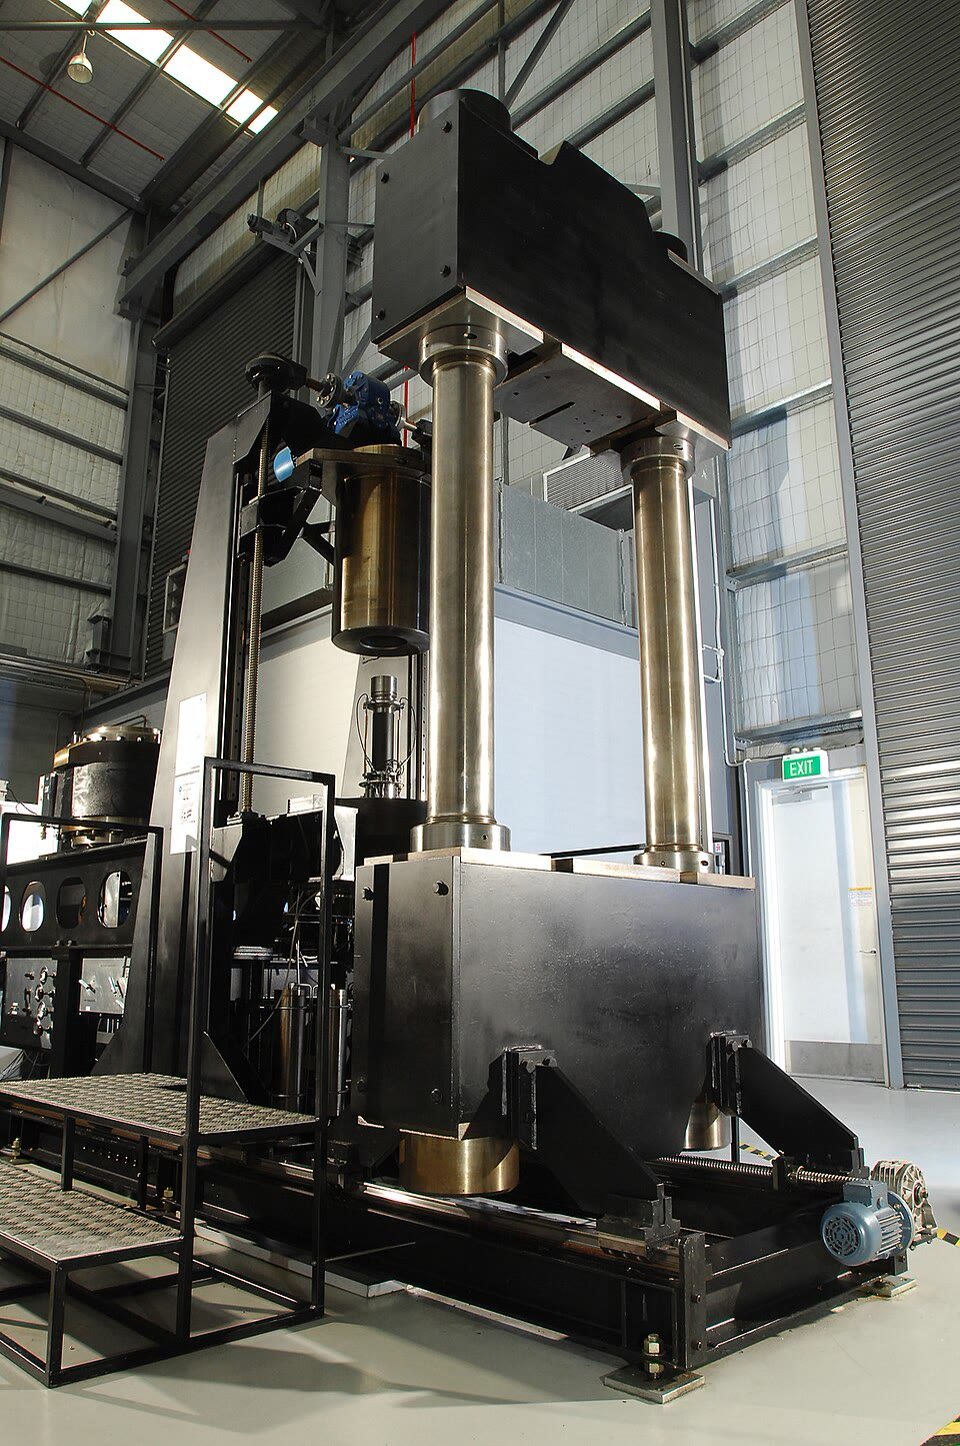
\includegraphics[width=\linewidth]{images/book3/b1-triaxial-cell.jpg}

{\scriptsize Een triaxiale cel met hoge druk om de sterkte van gesteente te meten (Darryl Peroni, CSIRO, CC BY 3.0).}
% ledger: commons:csiro-triaxial
\end{minipage}
\end{inthelab}

\section{De sterkte van de lithosfeer}\label{sec:b1:stress-strain-rheology:envelope}

Op elke diepte kan de \omterm{def:b1:layered-earth:lithosphere}{lithosfeer} op twee manieren bezwijken: door te schuiven langs breuken, met een sterkte die toeneemt met de effectieve druk, of door te kruipen, met een sterkte die afneemt naarmate het heter wordt. Zij vervormt op de manier die de kleinere spanning vraagt.

\begin{definition}[Sterkteomhullende, overgang bros--taai, seismogene laag]\label{def:b1:stress-strain-rheology:strength-envelope}
De \emph{sterkteomhullende}\index{sterkteomhullende} van de \omterm{def:b1:layered-earth:lithosphere}{lithosfeer} is de kromme, tegen de diepte, van de grootste \omterm{def:b1:stress-strain-rheology:principal}{differentiële spanning} die zij bij een gegeven reksnelheid kan dragen: op elke diepte de kleinere van de wrijvingssterkte en de kruipsterkte. De \emph{overgang bros--taai}\index{overgang bros--taai} is de diepte waarop die twee gelijk zijn: daarboven vervormt de rots door breuken, daaronder door kruip. De \emph{seismogene laag}\index{seismogene laag} is het dieptebereik waarin de meeste aardbevingen beginnen.
\end{definition}

\begin{proposition}[Wrijvingssterkte met de diepte]\label{prop:b1:stress-strain-rheology:brittle-gradient}
In een laag met dichtheid $\rho$, met een hydrostatische poriëndruk, één hoofdspanning verticaal, breuken van elke oriëntatie en zonder \omterm{def:b1:stress-strain-rheology:coulomb}{cohesie}, die met wrijving $\mu$ glijden, begint het glijden bij de \omterm{def:b1:stress-strain-rheology:principal}{differentiële spanning}
\begin{align*}
  \sigma_1 - \sigma_3 &= \frac{2\mu}{\sqrt{1+\mu^2} + \mu}\,\rho g z(1-\lambda)
  && \text{als $\sigma_v = \sigma_1$}, \\
  \sigma_1 - \sigma_3 &= \frac{2\mu}{\sqrt{1+\mu^2} - \mu}\,\rho g z(1-\lambda)
  && \text{als $\sigma_v = \sigma_3$},
\end{align*}
met $\lambda = \rho_w/\rho$: het eerste geval geeft normaalbreuken, het tweede overschuivingen.
\end{proposition}

\begin{proof}
De verticale \omterm{def:b1:stress-strain-rheology:lithostatic}{effectieve spanning} is $S = \rho g z - \rho_w g z = \rho g z(1-\lambda)$.
Met $C = 0$ en $k = \sqrt{1+\mu^2}$ zegt \cref{thm:b1:stress-strain-rheology:failure-angle} dat een breuk glijdt wanneer $r = \mu c'/k$, met $r$ de straal en $c'$ het middelpunt van de effectieve cirkel van Mohr. Als $\sigma_v = \sigma_1$, dan is $\sigma_1' = S$ en $c' = S - r$, dus $rk = \mu S - \mu r$ en $r = \mu S/(k+\mu)$. Als $\sigma_v = \sigma_3$, dan is $c' = S + r$ en $r = \mu S/(k-\mu)$. De \omterm{def:b1:stress-strain-rheology:principal}{differentiële spanning} is $2r$.
\end{proof}

Met $\mu = 0.85$ en $\rho = \qty{2700}{kg.m^{-3}}$ neemt $S$ toe met \qty{16.7}{MPa} per kilometer, en de wrijvingssterkte met \qty{13.1}{MPa} per kilometer onder uitrekking en \qty{61.3}{MPa} per kilometer onder compressie, bijna vijf keer meer: een \omterm{def:b1:layered-earth:layers}{korst} is veel gemakkelijker uit elkaar te trekken dan samen te duwen. Boven een effectieve \omterm{def:b1:stress-strain-rheology:stress}{normaalspanning} van \qty{200}{MPa} neemt de bovenste tak van de \omterm{prop:b1:stress-strain-rheology:byerlee}{wet van Byerlee} het over, en daalt de helling, bij compressie, tot ongeveer \qty{35}{MPa} per kilometer.
% computed in figdata/bachelor-1/strength_envelope.py (tested); ledger: byerlee:1975

\begin{omfigure}
\begin{tikzpicture}
\pgfplotsset{envaxis/.style={omrecord, omdepth, scale only axis, width=5.6cm, height=7.2cm,
  xmin=-1000, xmax=2500, ymin=0, ymax=80, xtick={-1000,0,1000,2000},
  ytick={0,10,...,80}, unbounded coords=jump,
  xlabel={differentiële spanning $\sigma_1-\sigma_3$ (MPa)},
  tick label style={font=\scriptsize}, label style={font=\small},
  scaled x ticks=false, xticklabel style={/pgf/number format/.cd, 1000 sep={\,}}}}
% computed in figdata/bachelor-1/strength_envelope.py; ledger: byerlee:1975, lopez:flow-laws, codata:R, prem:moho-average
\begin{axis}[envaxis, name=cont, ylabel={diepte (km)}, title={\small (a) continent, \qty{55}{mW.m^{-2}}}]
\addplot[fill=omLithGranite!45, draw=none] table[x=x, y=depth] {figdata/out/bachelor-1-strength_envelope-continental-outline.dat};
\addplot[omThm, line width=0.5pt, restrict x to domain=-1:2450] table[x=thrust, y=depth] {figdata/out/bachelor-1-strength_envelope-continental.dat};
\addplot[omThm, line width=0.5pt, restrict x to domain=-2450:1] table[x expr=-\thisrow{normal}, y=depth] {figdata/out/bachelor-1-strength_envelope-continental.dat};
\addplot[omDef, line width=0.5pt, restrict x to domain=-1:2450] table[x=ductile, y=depth] {figdata/out/bachelor-1-strength_envelope-continental.dat};
\addplot[omDef, line width=0.5pt, restrict x to domain=-2450:1] table[x expr=-\thisrow{ductile}, y=depth] {figdata/out/bachelor-1-strength_envelope-continental.dat};
\addplot[black, line width=1.0pt] table[x=x, y=depth] {figdata/out/bachelor-1-strength_envelope-continental-outline.dat};
\draw[black!60, dashed] (axis cs:-1000,35) -- (axis cs:2500,35);
\node[font=\scriptsize, anchor=south east] at (axis cs:2480,35) {Moho};
\draw[black, densely dotted] (axis cs:0,0) -- (axis cs:0,80);
\draw[black!70] (axis cs:660,13.7) -- (axis cs:1700,18) node[anchor=north, font=\scriptsize, align=center, text=black] {overgang\\ \qty{14}{km}};
\draw[black!70] (axis cs:1870,44.6) -- (axis cs:1950,53) node[anchor=north east, font=\scriptsize, align=center, text=black] {mantelovergang};
\node[font=\scriptsize, anchor=north, omThm] at (axis cs:1500,3) {compressie};
\node[font=\scriptsize, anchor=north, omThm] at (axis cs:-560,3) {uitrekking};
\node[font=\scriptsize, anchor=west, omDef] at (axis cs:40,31) {nat kwartsiet};
\node[font=\scriptsize, anchor=west, omDef] at (axis cs:300,66) {droge olivijn};
\end{axis}
\begin{axis}[envaxis, at={(cont.east)}, anchor=west, xshift=0.6cm, yticklabels={}, title={\small (b) oceaanbodem van \qty{60}{Myr} oud}]
\addplot[fill=omLithBasalt!45, draw=none] table[x=x, y=depth] {figdata/out/bachelor-1-strength_envelope-oceanic-outline.dat};
\addplot[omThm, line width=0.5pt, restrict x to domain=-1:2450] table[x=thrust, y=depth] {figdata/out/bachelor-1-strength_envelope-oceanic.dat};
\addplot[omThm, line width=0.5pt, restrict x to domain=-2450:1] table[x expr=-\thisrow{normal}, y=depth] {figdata/out/bachelor-1-strength_envelope-oceanic.dat};
\addplot[omDef, line width=0.5pt, restrict x to domain=-1:2450] table[x=ductile, y=depth] {figdata/out/bachelor-1-strength_envelope-oceanic.dat};
\addplot[omDef, line width=0.5pt, restrict x to domain=-2450:1] table[x expr=-\thisrow{ductile}, y=depth] {figdata/out/bachelor-1-strength_envelope-oceanic.dat};
\addplot[black, line width=1.0pt] table[x=x, y=depth] {figdata/out/bachelor-1-strength_envelope-oceanic-outline.dat};
\draw[black, densely dotted] (axis cs:0,0) -- (axis cs:0,80);
\draw[black!70] (axis cs:2003,38.2) -- (axis cs:1900,50) node[anchor=north, font=\scriptsize, align=center, text=black] {overgang\\ \qty{38}{km}};
\node[font=\scriptsize, anchor=west, omDef] at (axis cs:300,66) {droge olivijn};
\end{axis}
\end{tikzpicture}
\par\smallskip{\small \omterm{def:b1:stress-strain-rheology:strength-envelope}{Sterkteomhullenden} bij de reksnelheid \qty{e-15}{s^{-1}}. Rood: wrijvingssterkte volgens de \omterm{prop:b1:stress-strain-rheology:byerlee}{wet van Byerlee} met een hydrostatische poriëndruk, voor compressie (overschuiving, rechts) en uitrekking (normaalbreuk, links, als negatief getekend); blauw: de kruipsterkte van nat kwartsiet in de continentale \omterm{def:b1:layered-earth:layers}{korst} en van droge \omterm{def:b1:rock-forming-minerals:groups}{olivijn} in de \omterm{def:b1:layered-earth:layers}{mantel}; zwarte omlijning en arcering: de sterkte, de kleinere van de twee op elke diepte. (a) Een continent met een \omterm{def:b1:heat-budget:heat-flow}{oppervlakte-warmtestroom} van \qty{55}{mW.m^{-2}} en een \omterm{def:b1:layered-earth:layers}{korst} van \qty{35}{km} dik: sterke bovenkorst, zwakke onderkorst, sterke bovenste \omterm{def:b1:layered-earth:layers}{mantel}. (b) Oceaanbodem van \qty{60}{Myr} oud: één sterke laag, \qty{38}{km} dik bij compressie.}
\label{fig:b1:stress-strain-rheology:envelope}
\end{omfigure}

De figuur hierboven zet de twee sterkten samen voor twee lithosferen. Het continent heeft de geoterm van \cref{ch:b1:heat-budget} met een \omterm{def:b1:heat-budget:heat-flow}{oppervlakte-warmtestroom} van \qty{55}{mW.m^{-2}}, een \omterm{def:b1:layered-earth:layers}{korst} van nat kwartsiet van \qty{35}{km} dik, en daaronder droge \omterm{def:b1:rock-forming-minerals:groups}{olivijn}; de oceaanbodem is \qty{60}{Myr} oud, met de halfruimtegeoterm van hetzelfde hoofdstuk, en \omterm{def:b1:rock-forming-minerals:groups}{olivijn} van de zeebodem af naar beneden. De reksnelheid is \qty{e-15}{s^{-1}}. De \qty{35}{km} is de gemiddelde diepte van de \omterm{def:b1:layered-earth:discontinuity}{Moho} onder de continenten in het referentie-Aardmodel van \cref{ch:b1:layered-earth}.
% ledger: prem:moho-average

Onder het continent valt de \omterm{def:b1:stress-strain-rheology:strength-envelope}{overgang bros--taai} op \qty{13.7}{km} bij compressie, bij \qty{249}{\degreeCelsius}, en op \qty{17.1}{km} bij uitrekking. Een warmere \omterm{def:b1:layered-earth:layers}{korst} zou haar omhoogbrengen, een koudere haar omlaag duwen, omdat de kruipwet bij een gegeven spanning alleen van de temperatuur afhangt. De overgang is het sterkste niveau van de \omterm{def:b1:layered-earth:layers}{korst}.
Daaronder stort de sterkte in: op de \omterm{def:b1:layered-earth:discontinuity}{Moho}, bij \qty{527}{\degreeCelsius}, stroomt kwartsiet onder \qty{7.6}{MPa}, terwijl \omterm{def:b1:rock-forming-minerals:groups}{olivijn} bij dezelfde temperatuur ongeveer \qty{30000}{MPa} zou nodig hebben, zo ver boven de wrijvingssterkte dat de top van de \omterm{def:b1:layered-earth:layers}{mantel} weer bros is. Een tweede overgang volgt op \qty{44.6}{km} bij compressie. De onderkorst van dit model is een zachte laag tussen twee sterke: de ``jelly sandwich''. Onder de oceaan is de hele \omterm{def:b1:layered-earth:lithosphere}{lithosfeer} \omterm{def:b1:rock-forming-minerals:groups}{olivijn}, en neemt de sterkte toe tot aan één overgang op \qty{38.2}{km}, bij \qty{641}{\degreeCelsius}.
% computed in figdata/bachelor-1/strength_envelope.py (tested)

De aardbevingen stemmen overeen met de oceanische omhullende: binnen de oceanische platen bereiken zij diepten waar de temperatuur \qtyrange{600}{800}{\degreeCelsius} is, dicht bij de \qty{641}{\degreeCelsius} van de enkele overgang van het model. Diepere aardbevingen komen alleen voor waar de ene plaat onder de andere zinkt, tot meer dan \qty{700}{km} (\cref{ch:b1:active-margins}).
% ledger: jackson:jelly, usgs:deepest

De continentale \omterm{def:b1:layered-earth:layers}{mantel} is waar het beeld omstreden is. Ongeveer twintig jaar was de jelly sandwich de heersende opvatting, gebaseerd op laboratoriummetingen van droge \omterm{def:b1:rock-forming-minerals:groups}{olivijn} en op enkele aardbevingen waarvan men dacht dat ze onder de \omterm{def:b1:layered-earth:discontinuity}{Moho} lagen. In 2002 betoogde James Jackson dat zij moest worden verlaten: betere diepten toonden dat aardbevingen in de continenten beperkt zijn tot één laag, meestal de bovenkorst, soms de hele \omterm{def:b1:layered-earth:layers}{korst}, zonder overtuigende aardbevingen in de \omterm{def:b1:layered-earth:layers}{mantel} eronder, zelfs waar de temperatuur van de \omterm{def:b1:layered-earth:discontinuity}{Moho} slechts \qtyrange{300}{500}{\degreeCelsius} bedraagt. Kleine hoeveelheden water, enkele delen per miljoen in \omterm{def:b1:rock-forming-minerals:groups}{olivijn}, zijn genoeg om haar sterk te verzwakken, en de continentale \omterm{def:b1:layered-earth:layers}{mantel} kan wel zoveel bevatten; de sterkte van de continenten zou dan vooral in hun \omterm{def:b1:layered-earth:layers}{korst} liggen. De twee opvattingen trekken verschillende omhullenden uit dezelfde wetten, met droge of natte \omterm{def:b1:rock-forming-minerals:groups}{olivijn} onder de \omterm{def:b1:layered-earth:discontinuity}{Moho}.
% ledger: jackson:jelly
Hoe het ook zij, een omhullende is een grens en geen meting: de laboratoriumwetten worden geëxtrapoleerd over vele grootte-orden van reksnelheid, en de piekspanningen die zij toont, meer dan een gigapascal, liggen ver boven de \qtyrange{1}{10}{MPa} die aardbevingen blijken vrij te maken.
% ledger: jackson:jelly

\section{Oefeningen}

\begin{exercise}[$\star$]\label{exo:b1:stress-strain-rheology:1}
Neem een \omterm{def:b1:layered-earth:layers}{korst} met dichtheid \qty{2700}{kg.m^{-3}} en $g = \qty{9.81}{m.s^{-2}}$. Bereken op een diepte van \qty{10}{km} (a) de verticale spanning, (b) de hydrostatische poriëndruk, (c) de verticale \omterm{def:b1:stress-strain-rheology:lithostatic}{effectieve spanning} en de poriëndrukverhouding $\lambda$.
\end{exercise}

\begin{exercise}[$\star$]\label{exo:b1:stress-strain-rheology:2}
(a) Een laag van \qty{10}{km} lang wordt uitgerekt tot \qty{13}{km}: geef haar \omterm{def:b1:stress-strain-rheology:strain}{verlenging} en haar \omterm{def:b1:stress-strain-rheology:strain}{strekking}. (b) Een andere, \qty{10}{km} lang, wordt verkort tot \qty{7}{km}. (c) Twee lijnen van een rots die loodrecht stonden, maken nu een hoek van \ang{60}: geef de hoekschuif en de \omterm{def:b1:stress-strain-rheology:strain}{schuifrek}.
\end{exercise}

\begin{exercise}[$\star$]\label{exo:b1:stress-strain-rheology:3}
Op een punt zijn $\sigma_1 = \qty{100}{MPa}$ en $\sigma_3 = \qty{40}{MPa}$. (a) Teken de cirkel van Mohr. (b) Geef de grootste schuifspanning, de vlakken waarop zij werkt en de \omterm{def:b1:stress-strain-rheology:stress}{normaalspanning} op die vlakken. (c) Bereken $\sigma_n$ en $\tau$ op het vlak waarvan de normaal \ang{30} maakt met $\sigma_1$.
\end{exercise}

\begin{exercise}[$\star$]\label{exo:b1:stress-strain-rheology:4}
Een rots heeft de \omterm{def:b1:stress-strain-rheology:coulomb}{cohesie} \qty{10}{MPa} en de \omterm{def:b1:stress-strain-rheology:coulomb}{inwendige wrijvingshoek} \ang{30}. (a) Geef onder welke hoek met $\sigma_1$ zij breekt, en welke hoek de twee mogelijke breukvlakken met elkaar maken. (b) Bepaal, met $\sigma_3' = \qty{20}{MPa}$, de effectieve $\sigma_1'$ die haar breekt.
\end{exercise}

\begin{exercise}[$\star\star$]\label{exo:b1:stress-strain-rheology:5}
In de assen $x$ (horizontaal) en $y$ (verticaal) geldt $\sigma_{xx} = \qty{60}{MPa}$, $\sigma_{yy} = \qty{20}{MPa}$ en $\sigma_{xy} = \qty{15}{MPa}$. (a) Bereken de \omterm{def:b1:stress-strain-rheology:principal}{hoofdspanningen} en de hoek $\theta_p$. (b) Toon met \cref{prop:b1:stress-strain-rheology:transformation} aan dat het vlak met normaal $\theta_p$ geen schuifspanning draagt en dat de \omterm{def:b1:stress-strain-rheology:stress}{normaalspanning} erop $\sigma_1$ is. (c) Bepaal de grootste schuifspanning in dit punt.
\end{exercise}

\begin{exercise}[$\star\star$]\label{exo:b1:stress-strain-rheology:6}
Een schuifzone heeft haar gesteente vervormd door een \omterm{def:b1:stress-strain-rheology:shear-types}{eenvoudige schuif} $\gamma = 2$. (a) Bereken de hoofdstrekkingen en de hoek van de lange as van de \omterm{def:b1:stress-strain-rheology:strain-ellipse}{rekellips} met de schuifrichting. (b) Controleer dat het oppervlak niet is veranderd. (c) Een lijn van materiaal lag onder \ang{45} met de schuifrichting, stijgend in de zin van de schuif: waar ligt zij nu, en wat is haar \omterm{def:b1:stress-strain-rheology:strain}{strekking}? Vergelijk met (a).
\end{exercise}

\begin{exercise}[$\star\star$]\label{exo:b1:stress-strain-rheology:7}
In een schuifzone van \qty{200}{m} dik zijn kleine ronde vlekken in een lei ellipsen geworden met assen in de verhouding 4 tot 1. Neem een \omterm{def:b1:stress-strain-rheology:shear-types}{eenvoudige schuif} aan, zonder verandering van oppervlak. (a) Bepaal $S_1$, $S_2$ en $\gamma$. (b) Onder welke hoek met de wanden van de zone moeten de lange assen liggen? (c) Hoe ver is de ene wand langs de andere verschoven?
\end{exercise}

\begin{exercise}[$\star\star$]\label{exo:b1:stress-strain-rheology:8}
Een breuk op een diepte van \qty{3}{km}, in een \omterm{def:b1:layered-earth:layers}{korst} met dichtheid \qty{2700}{kg.m^{-3}}, draagt de \omterm{def:b1:stress-strain-rheology:stress}{normaalspanning} \qty{70}{MPa} en de schuifspanning \qty{30}{MPa}. (a) Ga na of zij volgens de \omterm{prop:b1:stress-strain-rheology:byerlee}{wet van Byerlee} glijdt bij een hydrostatische poriëndruk. (b) Doe hetzelfde als de poriën zijn afgesloten en $\lambda = 0.6$. (c) Bepaal de waarde van $\lambda$ waarbij zij begint te glijden.
\end{exercise}

\begin{exercise}[$\star\star$]\label{exo:b1:stress-strain-rheology:9}
Gebruik de kruipwet van nat kwartsiet (\cref{prop:b1:stress-strain-rheology:creep}). (a) Met welke factor moet de spanning stijgen om het tien keer sneller te laten stromen? (b) Met welke factor daalt de sterkte ervan tussen \qty{400}{\degreeCelsius} en \qty{500}{\degreeCelsius}, bij dezelfde snelheid en met $V = 0$? (c) Leg met deze twee resultaten uit waarom de diepte van de \omterm{def:b1:stress-strain-rheology:strength-envelope}{overgang bros--taai} veel meer van de geoterm afhangt dan van de reksnelheid.
\end{exercise}

\begin{exercise}[$\star\star\star$]\label{exo:b1:stress-strain-rheology:10}
Waar de verticale spanning $\sigma_2$ is, zijn de breuken strike-slip. Neem aan dat de verticale \omterm{def:b1:stress-strain-rheology:lithostatic}{effectieve spanning} dan het gemiddelde $(\sigma_1' + \sigma_3')/2$ is. (a) Toon aan dat glijden met wrijving $\mu$ en zonder \omterm{def:b1:stress-strain-rheology:coulomb}{cohesie} begint bij $\sigma_1 - \sigma_3 = 2\mu\,\rho g z(1-\lambda)/\sqrt{1+\mu^2}$. (b) Bereken de helling in megapascal per kilometer voor $\mu = 0.85$ en $\rho = \qty{2700}{kg.m^{-3}}$, en plaats haar tussen de hellingen van normaal- en overschuivingsbreuken. (c) Druk elk van de drie hellingen uit als een veelvoud van de verticale \omterm{def:b1:stress-strain-rheology:lithostatic}{effectieve spanning}.
\end{exercise}

\begin{exercise}[$\star\star\star$]\label{exo:b1:stress-strain-rheology:11}
Modelleer de oceanische \omterm{def:b1:layered-earth:lithosphere}{lithosfeer} van \qty{60}{Myr} oud als een halfruimte die is afgekoeld vanaf \qty{1350}{\degreeCelsius}, met een oppervlak op \qty{0}{\degreeCelsius} en
$\kappa = \qty{e-6}{m^2.s^{-1}}$: $T = \num{1350}\operatorname{erf}\bigl(z/(2\sqrt{\kappa t})\bigr)$.
(a) Bereken $2\sqrt{\kappa t}$. (b) Bepaal de diepten van de isothermen van \qty{600}{\degreeCelsius} en \qty{800}{\degreeCelsius}. (c) Vergelijk de diepten waar aardbevingen binnen de oceanische platen komen, namelijk waar de temperatuur \qtyrange{600}{800}{\degreeCelsius} is, met de \omterm{def:b1:stress-strain-rheology:strength-envelope}{overgang bros--taai} in de oceanische \omterm{def:b1:stress-strain-rheology:strength-envelope}{sterkteomhullende} van dit hoofdstuk, op \qty{38.2}{km} en \qty{641}{\degreeCelsius}.
% ledger: jackson:jelly
\end{exercise}

\begin{exercise}[$\star\star\star$]\label{exo:b1:stress-strain-rheology:12}
Een rots wordt doorsneden door breuken van elke oriëntatie, die alle de richting van $\sigma_2$ bevatten, zonder \omterm{def:b1:stress-strain-rheology:coulomb}{cohesie} en met wrijving 0.85. De effectieve \omterm{def:b1:stress-strain-rheology:principal}{hoofdspanningen} zijn $\sigma_1' = \qty{110}{MPa}$ en $\sigma_3' = \qty{20}{MPa}$. (a) Toon aan dat sommige breuken schuiven. (b) Bepaal het bereik van de hoek tussen de glijdende breuken en $\sigma_1$. Geef aan welke in het midden van het bereik ligt. (c) Tot welke waarde van $\sigma_1'$, met $\sigma_3'$ vast, schuift nog minstens één breuk?
\end{exercise}

\section{Probleem: glijdt de breuk?}

\begin{problem}[{Weekendprobleem --- de spanning op een normaalbreuk op een diepte van vijf kilometer, haar veiligheidsmarge en de stijging van de poriëndruk die haar tot schuiven zou brengen}]
\label{pb:b1:stress-strain-rheology:1}
% values: calc/ch16.py; ledger: byerlee:1975, hb81:denver
Een breuk loopt noord--zuid en helt \ang{60} naar het oosten. Een injectieput bereikt haar op een diepte van \qty{5.00}{km}, in een \omterm{def:b1:layered-earth:layers}{korst} met dichtheid \qty{2700}{kg.m^{-3}} waarvan de poriën met het oppervlak zijn verbonden. Een meting in de put geeft de horizontale spanning loodrecht op de breuk, \qty{75.0}{MPa}; de horizontale spanning langs de \omterm{def:b1:geological-maps:attitude}{strijk} ligt tussen die en de verticale spanning, zodat het probleem tweedimensionaal is in het verticale vlak oost--west. Neem $g = \qty{9.81}{m.s^{-2}}$, water met dichtheid \qty{1000}{kg.m^{-3}} en de \omterm{prop:b1:stress-strain-rheology:byerlee}{wet van Byerlee}. Geef spanningen tot op \qty{0.01}{MPa} nauwkeurig.

\medskip
\noindent\textbf{Deel I --- De spanningstoestand.}
\begin{enumerate}
  \item Bereken de verticale spanning op de diepte van de breuk.
  \item Bereken de hydrostatische poriëndruk daar, en de verhouding $\lambda$.
  \item Geef aan welke van de twee spanningen $\sigma_1$ is en welke $\sigma_3$, en welk soort breuk deze spanningstoestand aandrijft.
  \item Bereken de \omterm{def:b1:stress-strain-rheology:principal}{differentiële spanning}, het middelpunt en de straal van de cirkel van Mohr.
  \item Bereken de effectieve \omterm{def:b1:stress-strain-rheology:principal}{hoofdspanningen} en het middelpunt van de effectieve cirkel.
  \item Schrijf, met $x$ horizontaal naar het oosten en $y$ verticaal, de drie componenten $\sigma_{xx}$, $\sigma_{yy}$, $\sigma_{xy}$ op. Leg uit waarom $\sigma_{xy}$ nul is.
\end{enumerate}

\medskip
\noindent\textbf{Deel II --- De spanningen op de breuk.}
\begin{enumerate}[resume]
  \item Geef de eenheidsnormaal op de breuk in de assen van vraag 6, en de hoek $\theta$ tussen haar en $\sigma_1$.
  \item Bereken $\sigma_n$ en $\tau$ op de breuk met \cref{prop:b1:stress-strain-rheology:transformation}.
  \item Controleer beide waarden met de cirkel van Mohr en geef de hoek vanaf het $\sigma_1$-einde waaronder de breuk ligt.
  \item Bereken de effectieve \omterm{def:b1:stress-strain-rheology:stress}{normaalspanning} op de breuk.
  \item Bereken de verhouding $\tau/\sigma_n'$ en vergelijk haar met 0.85.
  \item Geef de schuifspanning die de breuk onder de huidige effectieve \omterm{def:b1:stress-strain-rheology:stress}{normaalspanning} tot schuiven zou brengen, en hoeveel megapascal zij tekortkomt.
\end{enumerate}

\medskip
\noindent\textbf{Deel III --- De cirkel van Mohr en de wet van Byerlee.}
\begin{enumerate}[resume]
  \item Teken de effectieve cirkel van Mohr en de lijn van Byerlee op schaal.
  \item Bereken de afstand van het middelpunt van de cirkel tot de lijn en vergelijk haar met de straal; geef aan of enig vlak door de rots kan schuiven.
  \item Welk vlak zou het eerst schuiven? Geef zijn hoek met $\sigma_1$ en zijn helling.
  \item Bereken met \cref{prop:b1:stress-strain-rheology:brittle-gradient} de \omterm{def:b1:stress-strain-rheology:principal}{differentiële spanning} waarbij normaalbreuken op deze diepte schuiven, en controleer haar tegen de helling van \qty{13.1}{MPa} per kilometer.
  \item Bepaal hoe laag de horizontale spanning moet dalen opdat het best georiënteerde vlak schuift.
  \item Bepaal hoe laag de horizontale spanning voor de breuk van het probleem moet zijn om te schuiven, en leg uit waarom zij lager is.
\end{enumerate}

\medskip
\noindent\textbf{Deel IV --- Injectie.}
\begin{enumerate}[resume]
  \item Leg uit waarom een stijging $\Delta P$ van de poriëndruk de effectieve cirkel met $\Delta P$ naar links verschuift zonder haar straal te veranderen.
  \item Bereken de stijging van de poriëndruk die het best georiënteerde vlak tot schuiven brengt.
  \item De put is vol water. Bepaal welke extra druk de pomp aan de bronkop moet uitoefenen om de poriëndruk op de breuk met die hoeveelheid te verhogen. Geef aan hoe hoog een waterkolom daarmee overeenkomt.
  \item Ga na of de breuk al zou glijden als de wrijving erop 0.6 was in plaats van 0.85. Leg uit wat de rust van de breuk over haar wrijving zegt.
  \item Bepaal bij welke verhouding $\lambda$ het best georiënteerde vlak schuift.
  \item Bepaal, op één decimaal en in megapascal, de stijging van de poriëndruk die deze breuk tot schuiven brengt.
\end{enumerate}
\end{problem}
